\documentclass[8pt,a5paper]{acm_proc_article-sp}
% fix umlauts
\usepackage[ngerman]{babel}
\usepackage[utf8]{inputenc} 
\usepackage[T1]{fontenc}  % Times new Roman
\usepackage{mathptmx}
\usepackage[]{blindtext}
\usepackage[a5paper, left=1.70cm, right=1.20cm, top=1.30cm, bottom=1.40cm]{geometry}
\usepackage{epstopdf}
% balance columns. original from acm doesn't work
\usepackage{balance}
% colors
\usepackage[compact]{titlesec}
\usepackage{natbib}
\titlespacing{\section}{0pt}{*0.7}{*0.5}

\usepackage[nolist]{acronym}
 
%\usepackage[usenames,dvipsnames]{xcolor}
\usepackage[greyscale]{xcolor} 
% automatic crosslinks
\usepackage[hyphens]{url}
\usepackage[colorlinks=false,
            allbordercolors={0 0 0},
            pdfborderstyle={/S/U/W 0.5}]{hyperref}
%glossaries
%\usepackage{makeidx}
%\makeindex
%\usepackage[nomain]{glossaries}
%\makeglossaries
%\makeindex

\newcommand{\glspl}[1]{{#1}}

% http://en.wikibooks.org/wiki/LaTeX/Glossary
% http://mirror.informatik.uni-mannheim.de/pub/mirrors/tex-archive/macros/latex/contrib/glossaries/glossariesbegin.pdf

% Definitionsliste
\newcommand{\defitem}[1]{\item[#1]\phantomsection\label{#1}\hfill\\} 
\newcommand{\defref}[1]{\hyperref[#1]{#1}} 
\newcommand{\rem}[1]{}
% Marking colors
\definecolor{todo}{rgb}{1,0.2,0.2}
\definecolor{reconsider}{rgb}{0.6,0.6,0.3}
\newcommand{\todo}[1]{{\color{todo} #1}}
\newcommand{\reconsider}[1]{{\color{reconsider} #1}}

% Hurenkinder und Schusterjungen verhindern
\clubpenalty10000
\widowpenalty10000
\displaywidowpenalty=10000


\graphicspath{{images/}{./}}

\title{Fahrerassistenzsysteme: Müdigkeitserkennung im Simulationsumfeld \titlenote{ \scriptsize \flushleft Betreuer Hochschule:  \  \ Prof. Dr. Martinez\\ \qquad \qquad \qquad \qquad \quad \ \  Hochschule Reutlingen\\ \qquad \quad \quad \quad \qquad \qquad \ \ Natividad.Martinez@Reutlingen-\\ \qquad \qquad \qquad \qquad \quad \ \ University.de\\  Wissenschaftliche Vertiefungskonferenz 2015\\ Wissenschaftliche Vertiefungskonferenz \\ 18. November 2015, Hochschule Reutlingen\\  \copyright 2015 Paul Pasler}}


\numberofauthors{3}
\author{
	\alignauthor
	  \center
		\aufnt{Paul Pasler}\\
          \affaddr{Reutlingen University}\\
        \textbf{\textsf{Paul.Pasler@Student.Reutlingen-University.DE}}
}



\begin{document}
\begin{acronym}
\acro{FAS}{Fahrerassistenzsystem}
\acro{FASs}{Fahrerassistenzsysteme}
\acro{ME}{Müdigkeitserkennung}
\acro{MESs}{Müdigkeitserkennungssysteme}
\acro{ADAS}{Advanced Driver Assistance System}
\acro{ADASs}{Advanced Driver Assistance Systems}
\acro{bspw}{beispielsweise}
\acro{RTU}{Reutlingen University}
\acro{BS}{Body-Sensoren}

\end{acronym}


\maketitle
\sloppypar{
\begin{abstract}
Mit Fortschreiten der Technik, verbreiten sich \acl{FAS}en immer weiter. Besonders der Teilbereich der \acl{ME} hilft schwere Unfälle zu vermeiden. Die \acl{ME} mit Body-Sensorik liefert sehr gute Ergebnisse, scheitert aber in der Praxis häufig auf Grund seines invasiven Charakters. Für die vorgelegte Arbeit werden Forschungsergebnisse aus diesem Bereich evaluiert und daraus im Simulationsumfeld der \acl{RTU}  ein Konzept entwickelt, dass Körperfunktionen überwacht und diese auswertet, ohne den Fahrer zu beeinträchtigen. Weiterhin wird die Möglichkeit einer einfachen Portierung der Anwendung vom Simulator in ein echtes Fahrzeug geprüft. Das vorgestellte Konzept, soll somit ein Höchstmaß an Genauigkeit, Tragekomfort und Mobilität vereinen.

\end{abstract}

\keywords{
\acf{ADAS}, \acl{FAS}, \acl{ME}
}

\category{A.0}{ACM}{
Experimentation
}


\section{Einleitung - WARUM?}
\label{chap:intro}
Fristeten \acl{FASs} vor wenigen Jahren ein Nischendasein in Oberklassewagen, werden sie immer günstiger und beliebter. Mittlerweile halten sie auch in Mittel- und Kleinwagen Einzug. Sie erhöhen den Komfort und helfen bei der Vermeidung schwerer Unfälle. Die \acl{ME} unterstützt dem Fahrer und rät ihm zu gegebenen Anlass eine Pause einzulegen. Laut dem Deutschen Verkehrssicherheitsrat zählt Müdigkeit, neben Geschwindigkeit, zu den häufigsten Unfallursachen und ist damit für jeden fünften schweren Unfall verantwortlich \cite{dvr_statistic}. In einer Studie der amerikanischen National Sleep Foundation, gab die Hälfte der Befragten an, dass sie schon einmal schläfrig gefahren seien und fast jeder dritte sogar kurz am Lenkrad eingeschlafen war. Dies zeigt die Wichtigkeit einer Erkennung von Müdigkeit und einer Meldung an den Fahrer \cite{nsf_statistic}. \\


\begin{figure*} 
  \begin{center}
    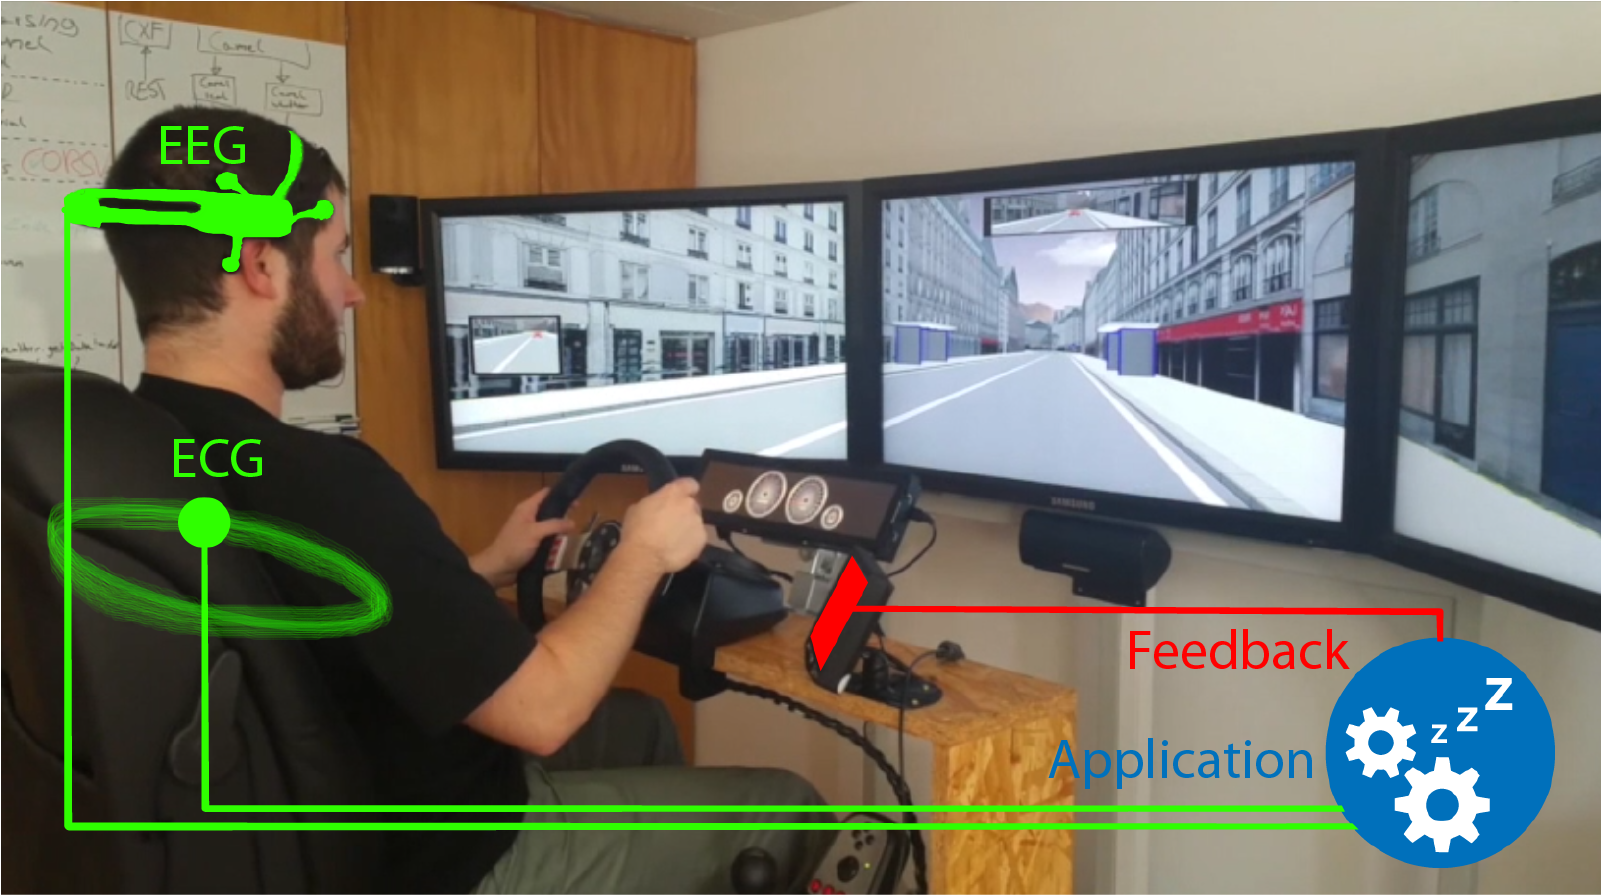
\includegraphics[width=12cm]{img/aufbau}
    \caption{Skizze des Systemaufbaus: \acl{BS} (EEG / EKG) liefert Daten an die Applikation und ein Feedback-Device warnt den Fahrer vor einfallender Müdigkeit. Bild zeigt den Fahrsimulator der \acl{RTU}.}
    \label{fig:sketch}
  \end{center}
\end{figure*}

Um das Risiko eines Unfalls auf Grund von Müdigkeit zu senken, soll langfristig ein multimodales System zu \acl{ME} entwickelt werden (Siehe Abb. \ref{fig:sketch}). Ziel dieser Arbeit ist es, aktuelle Arbeiten zu diesem Thema zu sichten und ein Konzept für ein solches System mit \acl{BS} zu erstellen. Die \acl{BS} messen Signale direkt am Körper und können somit sofort auf Veränderungen reagieren. Ein Algorithmus versucht an Hand der Messdaten herauszufinden, ob der Fahrer übermüdet ist und damit Gefahr läuft einen Sekundenschlaf zu bekommen. Es steht außer Frage, dass dieses System richtig und genau Warnen soll, sodass die Sicherheit zu jeder Zeit gewährleistet wird. Hierzu müssen die Signale aufbereitet und von Rauschen befreit werden. Da die Sensoren direkt am Körper anliegen, können sie den Fahrer beeinträchtigen. Das Problem der invasiven Sensoren soll weitestgehend eliminiert und den Fahrer wenig bis gar nicht beeinträchtigen. Feldversuche eignen sich nicht zur Entwicklung eines solchen Systems, da Eigen- und Fremdgefährdung eines übermüdeten Fahrers nicht vertretbar sind. Das System soll darum im Simulationsumfeld der \acl{RTU} entwickelt und getestet werden. Dennoch müssen die Ergebnisse einem Test im Straßenverkehr standhalten, da es unter Umständen zu anderen Signalen, \acl{bspw} aufgrund von erhöhtem Stress, kommen kann. Darum soll das System später leicht in ein echtes Fahrzeug portiert und validiert werden können. Gelingt dies, kann es weiterhin mit anderen Systemen gekoppelt zu werden, um das Gesamtergebnisse insgesamt zu verbessern. Damit hilft das vorgestellte Konzept, den Fahrer vor einer drohenden Müdigkeit zu warnen und so schwere Unfälle zu vermeiden.\\ 

Die Ausarbeitung gliedert sich folgendermaßen. Im Kapitel \ref{chap:me} werden verschiedene Forschungsergebnisse zur \acl{ME} aufgezeigt und in Kapitel \ref{chap:an} verglichen. Das Konzept eines portablen Systems zur \acl{ME} mit \acl{BS} wird im Kapitel \ref{chap:prop} vorgestellt. Der Versuchsaufbau und das Testszenario im Simulationsumfeld der \acl{RTU} ist Thema von Kapitel \ref{chap:eval}. Das Ergebnis und weitere Schritte werden in Kapitel \ref{chap:result} und \ref{chap:outro} beschrieben. In den anschließenden Absätzen werden Grundlagen für die kommenden Kapitel erläutert.

\section{Grundlagen}
In den folgenden Abschnitten werden Grundlagen für das Verständnis der weiteren Kapitel gelegt. Es wird ein grober Überblick zu \acl{FASs}, \acl{ME} und \acl{BS} gegeben.

\subsection{\acl{FASs}}
\acl{FASs} erhöhen dem Fahrer zum einen den Komfort und / oder die Sicherheit beim Fahren. So führen Einparkassistent,  Geschwindigkeitsregelanlage oder Navigation zu einer deutlich entspannteren Fahrt. Spurhalte-, Spurwechsel- oder Notbremsassistent wiederum unterstützen bei potentiell gefährlichen Manövern. Auch die \acl{ME} fällt in die zweite Kategorie (mehr dazu in Kapitel \ref{chap:me}).\\

Kompaß \cite{fasFuture} unterteilt \acl{FASs}, gemessen an der Reaktionszeit, in Planung, Führung und Stabilisierung. Hierbei fällt \acl{bspw} Navigation in die Planungsebene, da die Berechnung der Route mit unter mehrere Minuten brauchen kann. Auf Führungsebene werden dem Fahrer Empfehlungen und Warnungen innerhalb weniger Sekunden mitgeteilt, auf die er dann reagieren kann. Greift das System selbständig in den Fahrprozess ein, muss dies meist innerhalb von Millisekunden geschehen und dient oftmals zur Stabilisierungen, wie \acl{bspw} bei einem Fahrdynamik-Regelsystem.\\

Ein \acl{FAS} kann auf verschiedenste Arten mit dem Fahrer kommunizieren. Es handelt sich um eine klassische HCI-Schnittstelle. Am gebräuchlichsten, auch für sonstige Warnungen, sind schon seit längerem Optische und Akustische Signale. Aber auch Vibrationen in Lenkrad und Sitz zeigen gute Ergebnisse, wenn zwischen Signal und Nachricht ein Zusammenhang besteht (Bspw. Vibriert das Lenkrad bei verlassen der Spur).
\cite{Bertoldi:2010:MAD:2002368.2002370} beschreibt hierzu die verschiedenen Anwendungsgebiete und Unterschiede. \\

Jeder Automobilhersteller entwickelt mittlerweile seine eigenen \acl{FASs}. Datenerhebung (Sensoren), Berechnung und Kommunikation werden vom Fahrzeug selbst durchgeführt. Durch die Abschottung des Fahrzeugs sind Fahrzeugdaten nicht öffentlich zugänglich und können nur schwer von Außenstehenden genutzt werden. \\

Für wissenschaftliche Arbeiten bleibt entweder eine Kooperation mit Automobilherstellern oder das Ausweichen auf andere Devices, wie ein Smartphone und die Nutzung von Daten aus dem Internet (\acl{bspw} Kartendienste). Chen \cite{Chen:2015:ISV:2742647.2742659} und You \cite{You:2013:CAA:2462456.2465428} verfolgten diesen Ansatz. Smartphone bieten durch ihren hohen Verbreitungsgrad eine günstige Alternative zu eingebauten Systemen, können jedoch nicht auf Daten des Fahrzeugs zugreifen und müssen einfache Daten, wie \acl{bspw} Geschwindigkeit, selbst berechnen.

\subsection{\acl{ME}}
Die Erkennung von Müdigkeit kann wiederum auf ganz verschiedene Arten gelöst werden. Ein Ansatz versucht über Körpersignale herauszufinden, ob eine Müdigkeit bevorsteht. Wohingegen mit der Analyse des Fahrverhaltens das Selbe mit Sensoren an und im Auto realisiert wird.
Bei der Erkennung über Körpersignale, können wiederum \acl{BS} oder Computer-Vision-Techniken zur Überwachung des Fahrers genutzt werden. Zu unterscheiden ist weiterhin die physische und psychische Müdigkeit, welche sich jedoch beide negativ auf die Fähigkeiten des Fahrers auswirken. Alle Verfahren, die auf Senoren am Körper, die extra angezogen werden (bspw. ein Pulsmesser am Ohr, EEG) werden als inversive Verfahren bezeichnet. 

\begin{figure}[h] 
  \begin{center}
    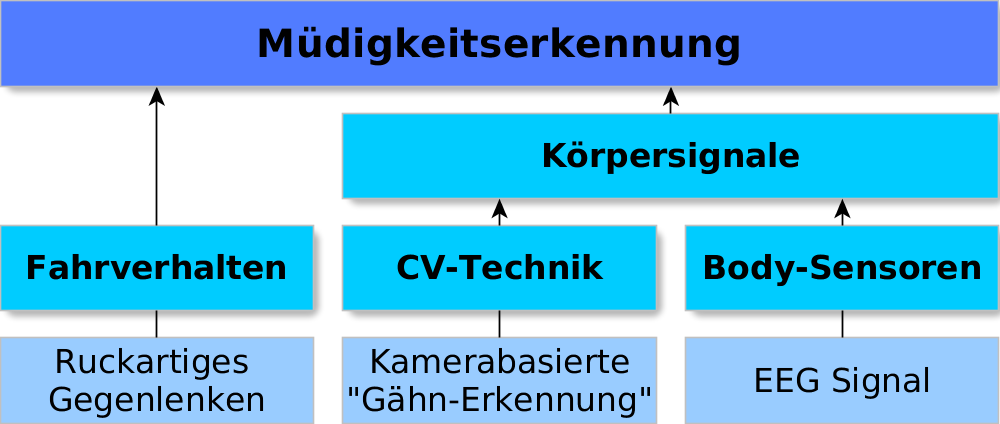
\includegraphics[width=6cm]{img/ddd}
    \caption{Einteilung der Systeme zur \acl{ME}}
    \label{fig:block}
  \end{center}
\end{figure}

Allen System gemein ist die Nutzung von Klassifizierungs- bzw. Machine-Learning-Algorithmen. Die gesammelten Daten geben nur Hinweise und sind kein Garant für eine Erkennung von Müdigkeit. \acl{MESs} wandeln hier auf einem schmalen Grad, da es zum einen um die Verhinderung schwerer Unfälle geht, zum anderen aber ein falsch auslösendes System die Akzeptanz vermindert und im schlimmsten Fall zu einer Deaktivierung führt. Um falsche Erkennungen weiter zu minimieren, werden oftmals mehrere Ansätze kombiniert.\\

In der Praxis setzen Automobilhersteller wie Daimler \cite{Daimler} und Volkswagen, sowie Automobilzulieferer wie Bosch \cite{Bosch} auf die Analyse des Fahrverhaltens. Insbesondere Spurhalten und ruckartiges Gegenlenken scheinen ein signifikantes Indiz für beginnende Übermüdung zu sein. Weiterhin sind externe Geräte und einige Apps für Smartphones erhältlich.

\subsection{\acl{BS}}
\acl{BS} messen verschiedenste Werte eines lebenden Körpers, wie den Puls, Temperatur oder Hirnwellen. Meistens werden sie direkt am oder im Körper eingesetzt.\\

Bei der Elektroenzephalografie (EEG) werden Elektroden auf der Kopfhaut angebracht und damit die Aktivität des Gehirns gemessen. Sie wird in der Medizin für die Diagnose von Epilepsie oder bei Komapatienten eingesetzt. Zudem findet sie in Schlaflabors Anwendung, um verschiedene Schlafphasen zu erfassen. Der Zusammenhang von Schlaf und Hirnaktivität kann auch bei der \acl{ME} in Fahrzeugen genutzt werden, um \acl{bspw} ein drohenden Sekundenschlaf zu erkennen \cite{Santamaria_eeg}. \\

Das Elektrokardiogramm (EKG) misst die Herzspannungskurve und stellt die Aktivität des Herzmuskels dar. So lassen sich vielfältige Aussagen über den Zustand des Herzens machen. Weiterhin können Herzrhythmus und -frequenz Hinweise auf eine einfallende Müdigkeit des Fahrers geben. Für die Messung des EKG Signals existieren mehrere Methoden, im medizinischen Bereich werden Elektroden an verschiedenen Körperstellen geklebt. Weiterhin werden, vor allem im Sport, Sensoren mit Gummibändern an Brust oder Handgelenk befestigt. \\

Eine weitere Möglichkeit Körperfunktionen aufzuzeichnen ist die Elektrookulografie (EOG). Hierbei kann die Bewegung der Augen bzw. das Ruhepotential der Netzhaut gemessen werden. Dazu werden Elektroden entweder rechts und links oder oben und unter dem Auge angebracht.\\

Grundlagen von \acl{FAS}, \acl{ME} und \acl{BS} waren Thema des vergangenen Kapitels. Für die Realisation von Systemen zur \acl{ME} existieren verschiedene Arbeiten, diese werden im nächsten Kapitel vorgestellt.

\section{Stand der Technik}
\label{chap:me}
Müdigkeit senkt die Konzentrationsfähigkeit des Fahrers, kann zu einer erhöhten Reaktionszeit und Fehleinschätzungen führen. So stellt es, unter anderem, der Deutscher Verkehrssicherheitsrat in einem Beschluss von 2009 \cite{DVR:Online} fest. Ursachen können wenig Schlaf, lange Fahrzeiten, Medikamente oder Alkohol sein.
Die \acl{ME} versucht an Hand verschiedener Daten und Sensoren, frühzeitig zu erkennen, ob der Fahrer gerade Anzeichen einer bevorstehenden Müdigkeit zeigt und empfiehlt eine Pause. Dabei soll nicht nur während eines Micro- oder Sekundenschlafs, sondern schon früher gewarnt werden. Hierfür existieren unterschiedliche Forschungsergebnisse, die im folgenden vorgestellt werden. Eine weitere Übersicht findet sich auch in \cite{Sahayadhas_121216937}.\\

Einige Ansätze beobachten den Fahrer und die Straße mit Hilfe von Kameras. Zhang et al. \cite{Zhang:2015:RSD:2753829.2629482} stellen hierzu eine Applikation mit der Verbindung eines Farb- und Tiefenbildes vor. Mit Hilfe einer Microsoft Kinect werden sowohl die Kopfpose, als auch die Augenstatus bestimmt. Um das System robuster zu gestalten, wird aus dem Farbbild,  zusätzlich zum Vorhandenen, das Tiefenbild berechnet. Mit der CarSafe App entwickleten You et al. \cite{You:2013:CAA:2462456.2465428} ein visuelles System zur Überwachung des Fahrers und der Straße. Hierfür genügt ein aktuelles Smartphone. Die App deckt hierbei neben der \acl{ME} auch andere Gefahrensituation (\acl{bspw} zu dicht Auffahren) ab. Es werden eine Analyse des Fahrers (Kopfpose und Augenstatus), sowie der Fahrweise kombiniert und der Fahrer gewarnt. Kamerabasierte Systeme sind angenehm für den Fahrer, da er keine weitere Hardware (Sensoren) installieren muss. Jedoch ist eine Kamera optischen Grenzen unterworfen, was den Einsatz bei Nacht oder schlechtem Wetter erschwert. Für eine \acl{ME} mit Smartphone, aber ohne Kameraeinsatz, könnte \acl{bspw} die App V-Sense \cite{Chen:2015:ISV:2742647.2742659} genutzt werden, da sie lediglich  eingebaute Sensoren nutzt.\\

Bundele and Banerjee \citep{Bundele:2009:DFV:1806338.1806478} zeigten, dass Müdigkeit über die elektrodermale Hautreaktion und Pulsoxymetrie erkannt werden kann. Die elektrodermale Hautreaktion (galvanische Hautreaktion, GSR) misst hierbei die Hautleitfähigkeit und hängt mit der Schweißproduktion zusammen. Bei der Pulsoxymetrie kann, durch ein optische Verfahren, die Sauerstoffsättigung des Blutes gemessen werden. In diesem Fall bedeutet eine geringere Sättigung ein erhöhtes Müdigkeitsgefühl. Diese Werte werden durch \acl{BS} ermittelt und werden mit einem Multi Layer Perceptron (MLP) klassifiziert. Interessant ist zudem der Einsatz von sogenannten Smart-Clothes (E-textiles), welche die Sensoren in der Kleidung eingearbeitet haben und somit zu ein Non-Inversiven Ansatz führen.\\

Park et al. \cite{Park:2009:DDD:1667780.1667798} beschränken sich in ihrer Arbeit auf die Analyse der Pulswelle durch Photoplethysmography (PPG), mit einem eingebauten Sensor am Lenkrad. Dies stellt schon ein größeren Eingriff in die Umgebung des Fahrzeugs dar, als es im Abschnitt zuvor der Fall war. Die Daten der PPG werden mit einer Support Vector Maschine (SVM) eingeordnet. Es zeigte sich, dass die Ausschlagshöhe des Puls ein gutes Mittel für die Erkennung von Müdigkeit darstellt. Um die Ergebnisse zu verbessern, wurde die entwickelte Software mit einem zuvor entwickelten visuellen System zur Kopfbewegung gekoppelt. \\

Zhang et al. \cite{zhang_6513058} befassten sich ebenfalls mit der Überwachung von Herzfunktionen, jedoch mit Hilfe eines EKGs. Sie fanden heraus, dass die Wavelet Packet Energie in bestimmten Frequenzbereichen auf eine Veränderung des QRS hinweist, welcher wiederum als Indiz für einfallende Müdigkeit genutzt werden kann. Dies erhöht nach ihren Angaben die Geschwindigkeit und die Genauigkeit der Erkennung. In Verbindung mit der Wavelet Entropie kann eine trainierte SVM nahezu 100\% erreichen. Rogado et al. \cite{Rogado_4913155} nutzen ebenfalls Daten aus dem EKG, um daraus die Herzfrequenzvariabilität (HFR, english HRV) zu berechnen und drohendes Einschlafen zu erkennen. Ähnliches Verhalten untersuchten Vicente et al. \cite{Vicente_6164509}. \\

Khushaba et al. \cite{Khushaba_5580017} versuchten das EKG Signal mit dem EEG Signal zu koppeln, um die Qualität der Erkennung zu verbessern. Sie verglichen die Erfolgsrate von EKG und EEG, sowie EOG und EEG. Sie nutzen hierfür einen "`fuzzy wavelet"' basierten Algorithmus und zeigten, dass das EEG, sowie die Kombination des EEG mit EKG oder EOG gute Ergebnisse liefert. Johnson et. al \cite{Johnson11} führten Versuche mit einem EEG und EOG durch. Mit der Diskriminanzanalyse zur Klassifizierung fanden sie heraus, dass das EEG alleine ausreicht und das EOG nicht benötigt wird. Wilson et al. \cite{wilson_890161} nutzten einen ähnlichen Ansatz, betrachteten jedoch von vornherein nur das EGG und versuchten die Klassifizierung mit einem Neuronalen Netzwerk durchzuführen. Sie hielten das Neuronale Netzwerk durchaus für geeignet, konnten aber kein brauchbares Ergebnis erzielen. Zu einem ähnlichen Ergebnis kamen Kahlifa et al. \cite{khalifa_893852}. Anders Subasi und Abdulhamit \cite{Subasi:2005:ARA:1707423.1707550}, sie konnten mit einer diskreten Wavelet-Transformation und einem Neuronalen Netz ein brauchbares Ergebnis erzielen. Sie konnten die Zustände Aufmerksam, Schläfrig (drowsy) und Schlafend mit jeweils über 90\% erkennen. Vuckovic et al. \cite{Vuckovic2002349} nutzen ebenfalls ein künstliches Neuronales Netz und machten hierzu verschiedene Versuche zum besten Algorithmus zur Erstellung des Netzes. Der Learning Vector Quantization lieferte bessere Ergebnisse, als der Widrow-Hoff Algorithmus und die Levenberg–Marquardt Regel. Im Vergleich zur Klassifizierung von EEG Experten, wurde mit ihrem System  eine über 90\% Übereinstimmung erreicht. Murthy und Khan \cite{Murthy_1} verbanden EEG Signale mit einer CV-Technik zur Augenliderkennung und nutzten hierfür ebenfalls ein Neuronales Netz. Mit Hilfe dieser multimodalen Daten, konnten 3 Status erkannt werden: Wach, Schläfrig und Schlafend.
Huang et al. \cite{Huang_548971} nutzten ein Hidden Markov Model für die Klassifizierung. Auch dieser Machnie Learning Algorithmus ist nach eigener Aussage geeignet, um aus einem EEG-Signal, passende Schlüsse für die \acl{ME} zu ziehen. Lin et al. \cite{Lin05eeg-baseddrowsiness} nutzten die Unabhängige Komponenten Analyse und Lineare Regression und konnten zeigen, dass hiermit eine Erkennungsrate von bis zu 88\% möglich ist.\\

Die Vielzahl an unterschiedlichen Arbeiten zum Thema \acl{ME} zeigt die Bandbreite der möglichen Umsetzungen und Kombinationen. Im kommenden Kapitel werden diese Analysiert und Verglichen.

\section{Vergleich / Analyse}
\label{chap:an}
Nach der Vorstellung der Arbeiten zu \acl{MESs}, werden diese nun bewertet und verglichen. Die Forschungsergebnisse werden nach den folgenden Kriterien überprüft: Genauigkeit, Komfort und Einsetzbarkeit.\\

Systeme die das Fahrverhalten analysieren und daraus Rückschlüsse auf den Wachheitsgrad des Fahrers ziehen, sind in der Praxis weit verbreitet. Die Sensoren sind im Fahrzeug fest verbaut und das System kann auf das jeweilige Fahrzeug abgestimmt werden. Hier liegt schon das erste Problem, da die Systeme nicht in einem Fahrzeug einer anderen Marke einsetzbar sind. Weiterhin finden sich im Internet viele Fragen zum Grund der Pausenempfehlung. Diese Systeme sind für normale Bedingungen genau und funktionieren gut. Dennoch finden sich im Internet mehrere Forenbeiträge, in denen die Nutzer fragen, wie diese Systeme funktionieren bzw. warum es zu Fehlalarmen kommt. Dies kann darauf hindeuten, dass die Erkennung für alle Bedingungen (Kurven, Unebenheiten auf der Straße) nicht einwandfrei arbeitet. Für den Fahrer sind diese Systeme jedoch sehr angenehm in der Nutzung, da er vom System nur dann etwas mitbekommt, wenn er vor Müdigkeit gewarnt wird. Da diese Systeme von vielen Automobilherstellern verwendet wird, lässt sich annehmen, dass \\

Videobasierte Systeme erfüllen ebenfalls ihren Zweck, sind aber leicht durch äußere Einflüsse, wie \acl{bspw} schlecht Lichtverhältnisse, beeinflussbar. Auch wenn Systeme mit Infrarotkameras diese Probleme vermindern, kann es sein, das \acl{bspw} Augen von (Sonnen-)Brillenträgern nicht richtig erkannt werden können.\\

Die meisten \acl{BS} liefern sehr gute Ergebnisse (+/- 90\%), es werden EEG, EKG, EOG und weitere Sensoren für die Datensammlung genutzt. Bei der Datenaufbereitung ist zu beachten, dass die elektrischen Signale anfällig für Störungen und Rauschen sind. Für die Klassifizierung wurde in den meisten Fällen eine Wavelet Transformation und ein Neuronales Netz verwendet. Weiterhin sind \acl{BS} wegen ihrer invasiven Eingenschaften (Die Sensoren liegen direkt am Körper an) weniger für den Serienbetrieb geeignet. Um dieses Problem zu lösen existieren bereits verschiedene Ansätze. So stellte der französische Automobilzulieferer seinen intelligenten Autositz "`Active-Wellness"' vor. Der Sitz ist mit passiven Sensoren ausgestattet und misst ständig den Herzrhythmus, die Atmung und weitere biometrische Daten, um bei einfallender Müdigkeit gegenzusteuern \footnote{\url{http://www.faurecia.de/node/1780}}. Auch Pulsmesser am Handgelenk werden immer besser, sind dabei nicht größer als eine Uhr und bieten ein vertretbaren Tragekomfort. \\

Aufgrund der hohen Genauigkeit von EEG, EKG und Co. sind diese Systeme zur Verbesserung oder Validierung anderer Systeme in der Testphase nützlich. Gelingt es zudem den invasiven Charakter gering zu halten oder gar ganz zu vermeiden, sind Systeme mit \acl{BS} auch für den Produktiveinsatz geeignet. Es bleibt zu zeigen, dass Genauigkeit und Tragekomfort im richtigen Verhältnis stehen. Hat sich ein System in der Simulationsumgebung bewährt, sollte das System in einem realen Fahrzeug getestet werden können.  \\

Die verschiedenen Ansätze zur \acl{ME} haben ihre Stärken und Schwächen. Arbeiten mit Körpersensoren zeigten bessere Ergebnisse als Systeme mit Kamera und Analyse des Fahrverhaltens. Im folgenden Kapitel wird dieser Ansatz daher für Entwicklung eines System zur \acl{ME} weiterverfolgt.

\section{Portables System zur \acl{ME} mit \acl{BS} - WAS?}
\label{chap:prop}
\textbf{machbarkeitsstudie, blockdiagram}\\
Wie im vorherigen Absatz gesehen, existieren sehr viele verschiedene Lösungen zur \acl{ME} in Fahrzeugen. Aufgrund der beschriebene Vorteile von \acl{BS}, soll das zu entwickelnde System jedoch mit eben diesen arbeiten und das Problem des Tragekomforts gelöst werden. Das vorgeschlagene System soll Genauigkeit, Tragekomfort und Portabilität maximieren (Siehe Abb. \ref{fig:emphasis}). \\

\begin{figure}[h] 
  \begin{center}
    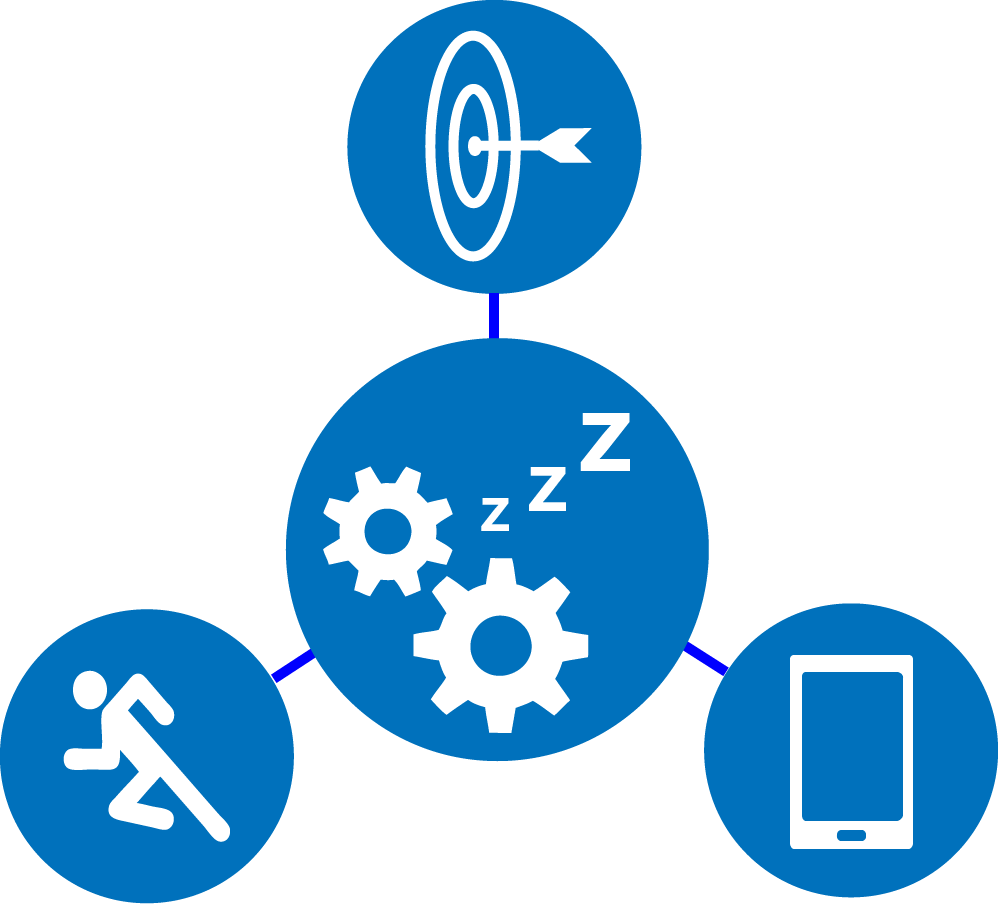
\includegraphics[width=4cm]{img/all}
    \caption{Schwerpunkte des Systems zur \acl{ME} (Im Uhrzeigersinn): Genauigkeit, Portabilität und Tragekomfort}
    \label{fig:emphasis}
  \end{center}
\end{figure}

EEG und EKG stehen in der Simulationsumgebung der \acl{RTU} zur Verfügung. Das System soll in der Lage sein, einfallende Müdigkeit zu erkennen und in angemessener Weise zu reagieren. Bei der Anwendung der Sensoren, soll insbesondere auf den Tragekomfort geachtet werden. Im besten Fall nimmt der Fahrer die Sensoren nicht wahr und wird durch diese nicht abgelenkt. Das EEG scheidet bei dieser Betrachtung von vorne herein aus und soll während der Entwicklung zur Verfeinerung bzw. Validierung genutzt werden. Im Bereich des EKGs existieren Lösungen mit höheren Tragekomfort. Diese liefern jedoch oftmals weniger gute Daten. Daher muss gezeigt werden, dass die Genauigkeit hoch und die Fehlerrate möglichst niedrig bleibt. 
Darum schlagen wir eine Umsetzung mit einem EKG Brustband (Siehe Kapitel \ref{subsec:sim}) vor, welches bei der Entwicklung von einem EEG validiert wird. Ein Austausch des Brustbandes durch einen Pulsmesser oder eine Smartwatch ist vorstellbar.\\

Tests mit übermüdeten Fahrern im Straßenverkehr lassen sich aus naheliegenden Gründen nicht durchführen. Die Fremd- und Selbstgefährdung ist deutlich zu hoch, auch wenn sich so die realistischsten Ergebnisse erzielen lassen. Auch die Durchführung in einem echten Fahrzeug und einem abgegrenzten Testgelände, würden zumindest ein Risiko für den Fahrer bedeuten. Darum bleibt meist nur eine Simulation, um das System zu \acl{ME} zu testen. Um im Fahrzeug verbaute Körpersensoren zu simulieren, werden die Sensordaten in der Simulationsumgebung mit dem CAN-Interface an die Anwendung übertragen, die Daten können aber auch direkt, ohne Simulator, übertragen werden. 
Dennoch sind Feldversuche ab einem gewissen Entwicklungsstand unumgänglich und sei es nur, um zu Prüfen, ob es in einer realen Testfahrt zu Fehlalarmen kommt (Stress, Beschleunigung oder Ähnliches). Darum muss die Anwendung sowohl im Simulator, als auch in einem realen Fahrzeug funktionieren und ohne großen Aufwand portiert werden können. Wenn dies gelingt, kann die Anwendung sowohl in unserem Simulator, einem realen Fahrzeug oder einem anderen Simulator genutzt werden, um dort etablierte Systeme zur \acl{ME} zu ergänzen oder zu validieren.
Das vorgestellte System muss demnach mit möglichst wenig Hardware auskommen und sich leicht auf andere Geräte portieren lassen. Im einfachsten Fall genügt ein Laptop oder Smartphone, einer Erweiterung auf einer Smartwatch ist vorstellbar.\\

Um das System auch zur Verbesserung oder Validierung anderer Systeme zur \acl{ME} zu nutzen, werden öffentliche Schnittstellen definiert und ein sauberes Logging der Daten implementiert. Die Daten der Überwachung sollen mit eindeutigem Zeitstempel versehen werden. So können sie mit anderen Daten, wie Videoaufzeichnung oder die anderer Systeme, zu einem späteren Zeitpunkt verglichen werden. \\

Erkennt das System eine drohende Müdigkeit, soll es den Fahrer über ein optisches oder akustisches Signal warnen. Das System soll mehrere Warnstufen zu kennen und je nach Müdigkeitsgrad reagieren. Ebenso wäre ein Rückmeldemechanismus vorstellbar, bei dem der Fahrer dem System einen Fehlalarm mitteilen kann. Diese Erweiterung ist jedoch mit Vorsicht zu genießen, da sich der Fahrer falsch einschätzen kann.\\

Die Anforderungen eines portablen Systems zur \acl{ME} mit \acl{BS} waren Thema des vergangenen Kapitels. Im folgenden wird das weitere Vorgehen, sowie Voraussetzungen zur Umsetzung beschrieben.

\section{Evaluationsplan - WIE?}
\label{chap:eval}
Um das zu entwickelnde System zu implementieren, müssen die notwendigen Schritte ausgearbeitet werden (Siehe Abb. \ref{fig:block}). Wichtige Bausteine sind die Datenaggregation der \acl{BS} und deren Anbindung in die Simulationsumgebung der \acl{RTU}. Die Datenaufbereitung und Klassifizierung sind weitere Teile Anwendung. Die Rückmeldung erkannter Müdigkeit ist der letzte Schritt. Bei der Evaluation müssen die Anforderungen Genauigkeit, Tragekomfort und Portierbarkeit beachtet werden. In den folgenden Absätzen werden hierzu Versuche und Voraussetzungen vorgestellt.

\begin{figure}[h] 
  \begin{center}
    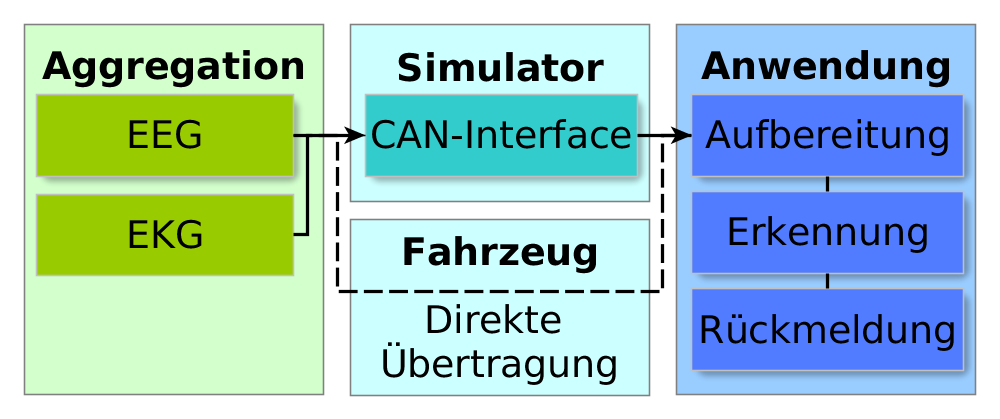
\includegraphics[width=5.5cm]{img/block}
    \caption{Der Ablauf der Datenströme und Aufgaben der Anwendung}
    \label{fig:block}
  \end{center}
\end{figure}

\subsection{Datenaggregation / Sensordaten}
Die Daten der genutzten EKG- und EEG-Sensoren müssen auf ihre Tauglichkeit geprüft werden. Dies kann unabhängig von Simulationsumfeld geschehen. Latenz oder Störsignale müssen beachtet und möglichst eliminiert werden. Ebenso muss die Aufbereitung der Signale erfolgen, sodass der Klassifizierer trainiert und getestet werden kann. Das kontinuierliche Signal muss im ersten Schritt in ein diskretes Signal umgewandelt werden. Dann können die Werte weiterverarbeitet werden, um ein aussagekräftiges Feature-Set zu erhalten.\\

Für das System wird ein EEG Epoc Emotiv \footnote{\url{https://emotiv.com/epoc.php}} und ein Brustband EKG Zephyr Bioharnes \footnote{\url{http://www.zephyranywhere.com/products/bioharness-3}} eingesetzt (Siehe Abb. \ref{fig:sensors}). Das EEG ist in der Simulationumgebung der \acl{RTU} bereits einsatzbereit. Die Anbindung des EKG Brustbands muss noch implementiert werden.

\begin{figure}[h] 
  \begin{center}
    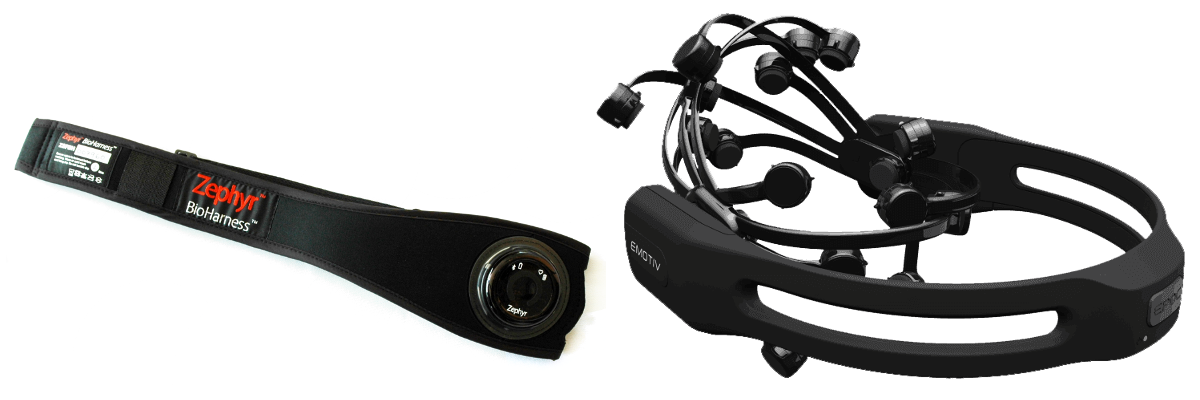
\includegraphics[width=6cm]{img/sensors}
    \caption{Links: EKG Brustband Zephyr Bioharnes; Rechts: EEG Epoc Emotiv}
    \label{fig:sensors}
  \end{center}
\end{figure}

\subsection{Anbindung in die Simulationsumgebung}
\label{subsec:sim}
Die Simulationsumgebung der \acl{RTU} ermöglicht es, Testfahrten unter möglichst realistischen Bedingungen zu durchzuführen (Siehe Abb. \ref{fig:architecure}). Sie ist ausgestattet mit einem Autositz, einem Lenkrad und Pedalen, sowie einer Gangschaltung. Weiterhin bringen drei $48^{\prime\prime}$ Monitore und ein Dolby-Surround-System einen audiovisuellen Eindruck einer Fahrsituation.\\

Auf technischer Ebene wird das System von drei Computer mit Leben gefüllt. Auf dem Simulations-Computer läuft die vom DFKI Saarbrücken entwickelte Software OpenDS \footnote{\url{http://www.dfki.de/web/aktuelles/aktuelles/cebit2013/opends}}. Hier können mehrere Karten und Konfigurationen eingestellt und getestet werden. Alle Simulationsdaten, werden via TCP/IP an den Daten-Computer gesendet. Dieser stellt die Daten über ein CAN-Interface zur Verfügung und loggt diese zusätzlich. Das CAN-Interface simuliert die Kommunikation mit dem Steuergerät eines realen Fahrzeugs. Der Anwendungs-Computer kann die CAN Daten über eine Schnittstelle empfangen und seine eigentliche Arbeit verrichten. Für Ein- und Ausgaben der Anwendung, befindet sich ein Touchscreen neben dem Lenkrad. Das System zur \acl{ME} wird auf dem Anwendungs-Computer ausgeführt.
\begin{figure}[h] 
  \begin{center}
    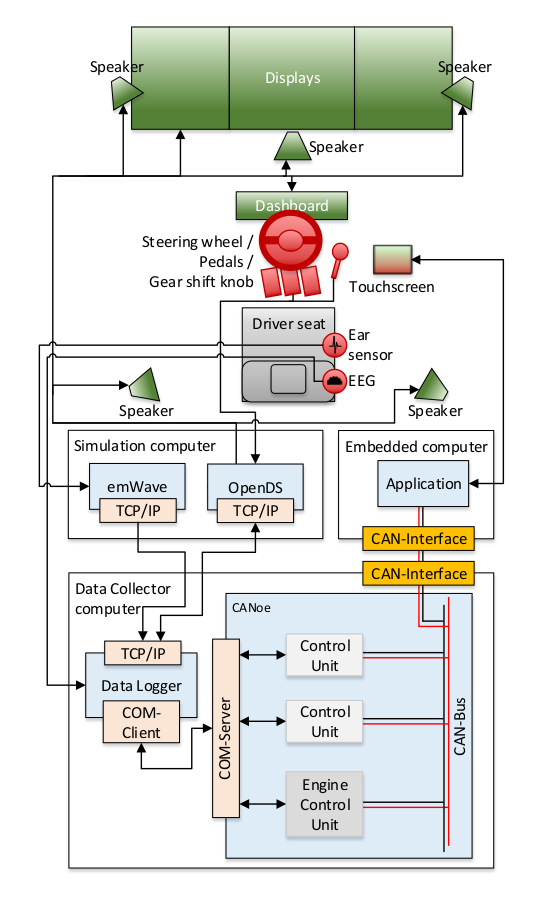
\includegraphics[width=6.5cm]{img/architecture}
    \label{fig:architecure}
    \caption[Aufbau des Simulators]{Der Aufbau des Simulators der \acl{RTU}}
  \end{center}
\end{figure}

\subsection{Algorithmen zur \acl{ME}}
Wie gesehen benötigt man für die Erkennung von Müdigkeit einen Machine-Learning-Algorithmus. In den betrachteten wissenschaftlichen Arbeiten wurde häufig auf Künstliche Neuronale Netzwerke vertraut \cite{wilson_890161} - \cite{Murthy_1}. Diese bilden ein vereinfachtes Modell des menschlichen Gehirns nach und wurden 1943 von Warren McCulloch und Walter Pitts entwickelt \cite{ann}.
Weiterhin werden Wavelet-Transformationen \cite{Chui:1992:IW:163196} zur Vorverarbeitung der Signale verwendet, um aus dem kontinuierlichen, ein diskretes Signal zu machen.

\subsection{Testszenario}
\label{sec:scene}
Das portable System zu \acl{ME} wird am Fahrsimulator der \acl{RTU} entwickelt und getestet.
Die Simulation kann jedoch nur ein Modell der Wirklichkeit sein und liefert nur eingeschränkte Ergebnisse. So konnten Blana et al. \cite{Blana_1} zeigen, dass sich das Fahrverhalten bei höheren Geschwindigkeiten im echten Straßenverkehr und im Simulationsumfeld unterscheidet. Engstrom et al.  \cite{Engstrom_2322937} konnten ebenfalls Unterschiede feststellen, zeigten jedoch auch, das Tests im Simulator dennoch valide Ergebnisse liefern können. \\

Um Daten mit einfallender Müdigkeit zu erhalten, muss ein passendes Szenario im Simulator erstellt werden. Es gilt beim Versuchsaufbau eine möglichst große Chance auf Sekundenschlaf bei den Probanden zu provozieren. Horne und Reyner legten nahe, dass die meisten Unfälle im Zusammenhang mit Schlaf in Großbritannien zwischen 02:00 - 06:00 und 14:00 - 16:00 passierten \cite{Horne_1757738}. Weiterhin lässt sich beobachten, dass Personen die 24 Stunden gar nicht oder nicht ausreichend (< 6h) geschlafen haben, deutlich anfälliger für Sekundenschlaf sind \cite{Peters_1}. 
Ein weiterer Faktor ist das Testszenario selbst. Es sollte möglichst gut erkennbar machen, ob der Proband gerade Fahrfehler macht und diese mit seinem Wachheitsgrad zusammenhängen. Weiterhin kann auch eine "`langweilige Teststrecke"' eine schnellere Ermüdung begünstigen. Langes geradeaus fahren und wenig Abwechslung sind zwar langweilig, aber nicht sehr anstrengend, darum sollte es eine Aufgabe sein, die den Probanden über die ganze Zeit fordert. Auch die Länge der Fahrt spielt eine Rolle, je länger die Fahraufgabe dauert, desto größer die Chance auf das Eintreten einer einfallenden Müdigkeit. \\

Vorstellbar ist somit folgender Ablauf: 1) 10min Einführung und Fahrsimulator ausprobieren. 2) 10min Straßenverkehr mit anderen Verkehrsteilnehmern unter Beachtung der Straßenverkehrsregeln. 3) 20min Gerade aus fahren und Spur halten 4) 10min Wiederholung von Schritt 2. 5) 10min Befragung und Selbsteinschätzung.
Im besten Fall lassen sich bei der Spurhalte-Aufgabe gegen Ende mehr Fahrfehler beobachten. Weiterhin sollte der Fahrer in Schritt 4) ein Unterschied zu Schritt 2) feststellen lassen.\\

In den vergangenen Abschnitten wurde die Vorgehensweise und weitere Schritte näher erläutert. Im kommenden Kapitel werden die Ergebnisse zusammengefasst und bewertet.


\section{Ergebnis}
\label{chap:result}
Die Erkennung von Müdigkeit stellt einen wichtigen Beitrag zu Sicherheit im Straßenverkehr dar. Schwere Unfälle können mit einem solchen System verhindert werden. Dazu ist es notwendig, möglichst früh und präzise eine drohende Müdigkeit zu erkennen. Für die Erkennung existieren verschiedene Ansätze, die sich in VR-basierte, Fahrverhaltenanalysierende und Body-Sensor-basierte Systeme einteilen lassen. \\

Systeme mit \acl{BS} zeigten sehr gute Ergebnisse, da sie kleinste Veränderungen von Körpersignalen direkt erkennen können. VR und Fahrverhalten können lediglich Folgen von Müdigkeit erkennen und reagieren damit potentiell später. Körpersensoren liegen meist direkt am Körper an und können den Fahrer während der Fahrt stören. Diese invasive Eigenschaft wurden möglichst gering gehalten und Vorschläge für weitere Verbesserungen unterbreitet (Smartwatch). Das Brustband stellt vermutlich einen guten Kompromiss von Tragekomfort und Genauigkeit dar. Ob die Genauigkeit des Sensors für eine frühzeitige Erkennung ausreicht, wird mit Hilfe eines EEGs belegt werden müssen.\\

Tests mit übermüdeten Fahrern sind im Straßenverkehr zu gefährlich, daher wird das System im Simulatorumfeld der \acl{RTU} durchgeführt. Dennoch muss das System in einem echten Fahrzeug einsetzbar sein und somit ohne größeren Aufwand portierbar sein. Dafür kann das System, samt \acl{BS}, vom Simulator entkoppelt werden und benötigt lediglich einen Laptop evtl. auch nur ein Smartphone. Das Einsatzgebiet des Systems liegt dabei nicht nur in einem echten Fahrzeug, sondern auch in der Verwendung in anderen Simulatoren. So kann es mit anderen Systemen zur \acl{ME} gekoppelt werden, um die Erkennungsraten zu verbessern.
Zur Entwicklung des Systems werden zudem geeignete Testdaten benötigt, Kapitel \ref{sec:scene} beschreibt den Ablauf eines solchen Testszenarios.


\section{Fazit und Ausblick}
\label{chap:outro}
Wie gesehen

Im nächsten Schritt wird es darum gehen, das vorgestellte Konzept umzusetzen. Dazu bleibt zu klären, ob das EKG Brustband ausreichend genaue Daten liefert. In Verbindung mit dem EEG muss ein passender Machine-Learning Algorithmus gefunden werden, der die Klassifizierung und \acl{ME} durchführt. Das vorgestellt Szenario muss durchgeführt werden. Funktioniert die Erkennung im Simulationsumfeld, muss das System Schrittweise verkleinert (Hardware- und Softwareseitig) und vom Simulator entkoppelt werden. Dann können erste Tests in einem echten Fahrzeug stattfinden. Das System soll in der weiteren Entwicklung mit anderen Systemen zu \acl{ME} verglichen werden und ggf. an einer Kopplung der Anwendungen gearbeitet werden.\\

In der letzten Ausbaustufe, ist vorstellbar, dass das System komplett in einer Smartwatch mit Pulsmesser läuft. Damit wäre die Anwendung mit keinerlei Beeinträchtigung des Fahrers verbunden. Ob die Sensorgenauigkeit und die Rechenleistung der Smartwatch ausreicht, bleibt zu zeigen.


\balance
\bibliographystyle{unsrt} % abbrv, alpha, plain, unsrt, apalike
\bibliography{Quellen}


\end{document}
